\section{Simterpose et son fonctionnement}
Simterpose est l'API qui va nous permettre d'intercepter les communications de
l'application avec la machine sur laquelle elle s'exécute. Sans cela,
l'application se rendrait compte que l'environnement réel ne correspond pas
celui dans lequel elle pense s'exécuter.

\subsection{Interception des actions}
 Une application distribuée peut vouloir communiquer avec l'hôte soit pour
 effectuer des calculs (SEB), soit pour communiquer avec d'autres applications
 sur le réseau. Quand Simterpose intercepte une communication venant d'un des
 processus d'une application, il modifie les caractéristiques de cette dernière
 pour qu'elle puisse s'exécuter sur la machine hôte. Quand la machine hôte
 renvoie une réponse à l'application, Simterpose l'intercepte également et la
 modifie pour que l'application ne voit pas le changement d'architecture. En
 même temps, il envoie au simulateur des données concernant le temps d'exécution
 de l'action sur la machine hôte pour calculer le temps sur la machine simulée
 puis envoie ce temps à l'application en plus du résultat afin de mettre à jour
 son horloge. Ainsi les calculs sont réellement exécuter sur la machine, les
 communications réellement émises sur le réseau géré par le simulateur et c'est
 le temps de réponse fourni par le simulateur qui va influencer l'horloge de
 l'application permettant ainsi d'imiter un environnement distribué. Finalement
 les applications ne communiquent plus directement entre elles puisque toute
 communication est interceptée par Simterpose puis gérée par le simulateur qui
 s'occupe du réseau.

{\color{red} MEttre un schéma de action interceptes, test modifie, renvoie,
  attrape reponse, simulateur, retour application}

Les délais calculés par le simulateur sont soit des temps de calculs soit des
temps de connexion. Les actions éxécutées par l'application peuvent-être soit
de simples calculs soit des requêtes de connexion ou communication réseau.

Pour intercepter ces actions, il faut d'abord choisir ce qu'on intercepte
exactement et avec quel outil. En effet une application peut communiquer avec le
noyau via différentes abstractions. Elle peut soit utiliser les fonctions
d'interraction directe avec le noyau que sont les appels systèmes, soit utiliser
les différentes abstractions fournies par le système d'exploitation:
bibliothèques (fonctions systèmes de la libc par exemple) ou les fonctions POSIX
dans le cas d'un système UNIX.

\begin{figure}[H]
 \centering
 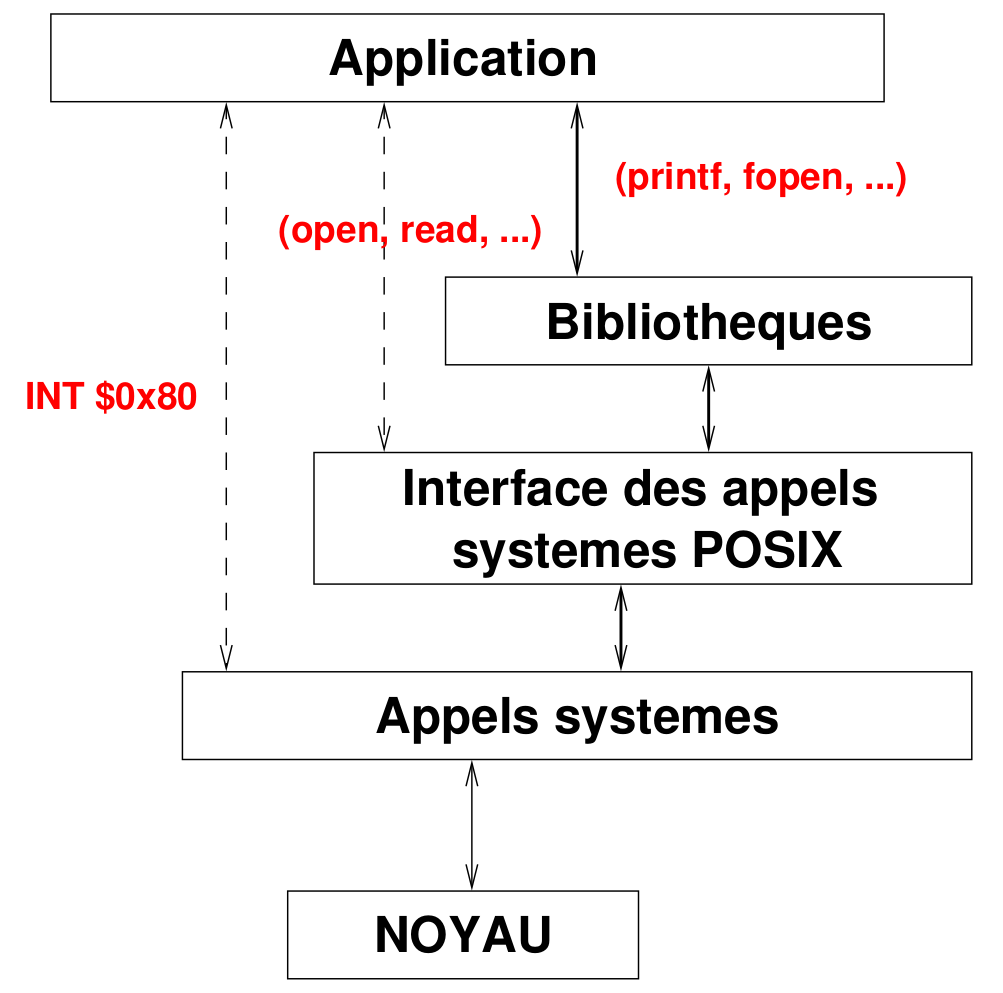
\includegraphics[scale=0.20]{Pictures/Communication_application_noyau.png}
 \caption{Communications possibles entre le noyau et une apllication}
 \label{AS_Communication}
\end{figure}


%Dans la figure~\ref{étiquette} page~\pageref{étiquette}
blabla sur pk plus logique prendre le plus bas donc on va voir ptrace
 liste... tout seul tout seul puis le lien entre
les deux
\subsection{Appel système: ptrace}
Nous allons intercepter les actions que sont les appels systèmes faits par
l'applciation, ainsi nous sommes sûr d'intercepter tous les types de
communications que l'application est susceptible d'initier avec le noyau. Les
appels systèmes sont constitués de deux parties; la première, l'entrée,
initialise l'appel via les registres de l'application qui contiennent les
arguments de l'appel puis donne la main au noyau. La seconde, la sortie, inscrit
le retour de l'appel système dans le registre de retour de l'application, les
registres d'arguments contennant toujours les valeurs reçues à l'entrée de
l'appel système, et rend la main à l'application. Nous devons donc intercepter
les deux parties de l'appel système pour maintenir notre environnement simulé et
donc stopper l'application à chaque fois pour récupérer ou modifier les
informations nécéssaires avant de lui rendre la main pour entrer ou sortir de
l'appel système.

Pour faire cela il existe de nombreux outils de différents types. Il y a l'API
ptrace, qui est lui même un appel système et qui permet de tracer tous les
événement désirés d'un processus contrôlé. Néanmoins ce dernier fait de nombreux
changements de contexte pour intercepter des événements. De plus il gère mal les
processus quand on a du multithreading, et il ne fait pas parti de la norme
POSIX donc son exécution peut varier d'une machine à une autre. On trouve
ensuite les API noyau aussi appelées modules d'instrumentations telles que:
utrace, kprobes, uprobes{\color{red}citation}. Utrace fait la même chose que
ptrace mais en mode noyau. Cela permet d'éviter les nombreux changements de
contexte pour gérer l'appel système et que le noyau l'exécute {\color{green}
  clair?}. De plus il gère les événements de thread et non de processus comme
ptrace ce qui évite le problème de gestion du multhreading. Kprobes quant à lui
permet à un utilisateur d’insérer dynamiquement des points d'arrêts à des
endroits spécifiques du noyau, dans notre cas ce serait le code des appels
systèmes. Ainsi l’utilisateur peut fournir un handler particulier à exécuter
avant ou après l’instruction marquée. Quand un point d'arrêt est touché kprobe
prend la main et exécute le bon handler. Uprobes fait la même chose que kprobes
mais pour le code d'applications et pas le code du noyau. Ainsi pour chaque
point d'arrêt géré par uprobes on doit créer un module noyau qui contient le
handler à exécuter quand le point d'arrêt est atteint. Uprobes utilise utrace
pour savoir quand on atteint ou non un point d'arrêt. Les deux avantages des API
noyau est qu'elles sont rapides et qu'elles ont accès à toutes les ressources
sans aucune restriction, mais ce dernier point représente aussi leur plus gros
défaut de par sa dangerosité. De plus, dans notre cas il ne semble pas judicieux
de modifier le code du noyau ou de faire de la programmation noyau via des
modules dont il faudra également gérer le bon chargement. Malgrè ses défauts
c'est donc l'appel système ptrace qui a été choisi. Maintenant que nous savons
pourquoi nous allons utiliser ptrace comme intercepteur pour les appels systèmes
nous allons étudier son fonctionnement.

Pour intercepter les éventuels appels systèmes d'une applciation nous allons
donc utiliser l'appel système \textbf{ptrace}{\color{red}citation}. Il permet de
controler l'exécution de processus mais également d'écrire et de lire
directement dans l'espace d'adressage d'un processus. Pour cela on créé deux
processus; un qui exécutera l'application et qu'on souhaite contrôler, on
l'appellera ``processus espionné'' et un autre qui le contrôlera appelé
``processus espion''. Le processus espionné indiquera au processus espion qu'il
souhaite être contrôlé via un appel système ptrace. À la reception de cet appel
le processus espion notifiera son attachement au processus espionné via un autre
appel à ptrace. Il indiquera également sur quelles actions du processus espionné
il veut être notifié, définissant ainsi les actions bloquantes pour le processus
espionné. Dans notre cas, ce seront les appels systèmes que l'on considérera
comme point d'arrêt pour le processus espionné. Ainsi quand un des processus de
l'application voudra faire un appel système quelconque il sera bloqué avant de
l'exécuter, l'appel système ptrace sera lancé et notifiera le processus
espion. Ce dernier fera les modifications nécessaires dans les registres du
processus espionné pour conserver la virtualisation de l'environnement, puis il
rendra la main au processus espionné bloqué pour que l'appel système puisse
avoir lieu. Au retour de l'appel système le processus espionné sera de noveau
stoppé, un ptrace sera envoye au processus espion qui remodifiera les
informations nécessaires. Puis il rendra la main au processus espionné bloqué
qui sortira de son appel système avec un résultat exécuté sur la machine hôte et
un temps d'exécution et une horloge fournie par le simulateur.

{\color{red} \textbf{gérer cette transition}} Néanmoins il a été montré dans un
précédent stage que l'appel système ptrace est inefficace voir inutile en ce qui
concerne tous les appels systèmes temporels qu'une application voudrait
faire. \textit{les appels systèmes ``time'', ``clock\_gettime'',
  ``gettimeofday'' avec \textbf{ptrace} ne sont pas possibles, d'où l'alliance
  avec LD\_PRELOAD} Par exemple lors d'un gettimeofday l'appel système n'est pas
lancé on répond directement au niveau de la bibliothèque ainsi on n'arrive même
pas au niveau de l'appel système, donc ptrace ne fait rien.  Problème
portabilité {\color{red} \textbf{gérer cette transition}}

\subsection{Variable d'environnement: LD\_PRELOAD}
On pourrait alors penser qu'une bonne solution serait d'intercepter les actions
de l'application au niveau des bibliothèques.{\color{red} rajouter des trucs sur
  VDSO}. Pour cela il existe la variable d'environnement \textbf{LD\_PRELOAD}
qui contient la liste des bibliothèques à précharger et qui est utilisée par le
noyau lors du premier lancement d'un programme. En effet par défaut Linux
effectue une édition de lien dynamiqe, l'édition de lien statique n'étant
choisie qu'en l'absence de bibliothèques partagées définissant les fonctions
utilisées par l'application. On va donc créer notre propre bibliothèque de
fonctions surchargeant chaque fonction susceptible d'être utilisée par
l'application. Une fonction surchargée contiendra alors toutes les modifications
nécessaires pour maintenir notre environnement simulé suivi de l'appel à la
fonction initiale puisqu'on souhaite juste intercepter l'appel et pas
l'empêcher. On préchargera cette bibliothèque avant les autres en la plaçant
dans la variable LD\_PRELOAD, ainsi nos fonctions passeront avant les fonctions
des bibliothèques usuelles.

Néanmoins si l'application fait un appel système directement sans passer par la
couche \textit{Bibliothèques} Fig.~\ref{AS_Communication} notre mécanisme
d'interception est countournée. En effet on ne peut surcharger que des fonctions
avec cette solution, pas des appels sytèmes. De même si on oublie de réécrire
une fonction d'une des bibliothèques utilisée par l'application. Cette solution
n'est donc pas suffisante pour le modèle d'interception que nous souhaitons
avoir.

Cependant on peut voir que LD\_PRELOAD résout les problèmes de ptrace concernant
les fonctions de temps, et inversement puisque ptrace permet d'intercepter les
appels systèmes que le modèle d'interception avec LD\_PRELOAD ne permet pas de
gérer. Une solution choisie lors d'un précédent stage est donc d'allier les
deux. On surchargera les fonctions temporelles dans notre bibliothèque
préchargée avec LD\_PRELOAD pour pallier les lacunes temporelles de ptrace. Et
pour toutes les autres fonctions ptrace s'en occupera, ainsi on est certain de
n'oublier aucune fonction. Maintenant que nous savons ce que nous devons
intercepter et comment l'intercepter nous allons voir ce que nous devons
modifier pour pouvoir maintenit notre émulation simulation.

\textit{Pour faire face à ce problème il a été choisi d'utiliser l'éditeur de
  lien dynamique \textbf{LD\_PRELOAD}, ce dernier intercepte les appels de
  l'application au niveau des bibliothèques. Pour cela on va créer une
  bibliothèque.}

\subsection{Modification à effectuer}
Lorsque ptrace est appelé en entrée ou sortie d'appel système, les modifications
à apporter ne sont pas forcément les mêmes selon qu'il s'agit d'une action
nécessitant l'utilisation du réseau ou non. Dans le cas d'un simple calcul ce
qu'il faut maintenir pour l'application, c'est une vision du temps correspondant
à celle qui s'écoulerait si elle était vraiment sur la machine simulée. Ainsi en
entrée d'appel système on n'a pas besoin de modifier quoique ce soit, par contre
au retour il faut modifier le temps d'exécution du calcul en le remplaçant par
celui calculé par le simulateur. Dans le cas d'une communication réseau il faut
gérer la transition entre réseau local et réseau simulé. En effet l'application
possède une adresse IP et des numéros de ports ``virtuels'' qui ne correspondent
pas forcément à ceux attribués dans le réseau local. De plus on ne peut pas se
baser uniquement sur les numéros de \textit{file descriptor} associé à une
socket pour identifier deux entités qui communiquent entre elles.En effet ces
\textit{file descriptor} sont uniques pour chaque socket d'un processus, mais
plusieurs processus peuvent avoir un même numéro de \textit{file descriptor}
pour des sockets de communicatiosn différentes puisque chacune à son propre
espace mémoire. Pour pallier à ce probème on va utiliser en plus du numéro de
socket, les adresses IP et les ports locaux et distants des deux entités qui
souhaitent communiquer comme moyen d'identification. Pour gérer toutes ces
modifications deux solutions ont été proposées lors d'un précédent stage: la
``médiation par traduction d'adresse'' et la ``full mediation''.

{\color{red}schéma}
\paragraph{Traduction d'adresse}
 Avec ce type de médiation on considère que le noyau gère des
 communications. Ainsi en entrée et sortie d'appel système Simterpose va juste
 s'occuper de la transition entre réseau ``virtuel'' et réseau local. Pour cela
 Simterpose gère un tableau de correspondance, dans lequel pour chaque
 application on a un couple (adresse IP et des ports ``virtuels'', adresse IP et
 ports ``réel'' sur le réseau).  De fait en entrée de l'appel système,
 Simterpose devra remplacer l'adresse et les ports ``virtuels'' de l'application
 par l'adresse et les ports réels sur le réseau local, ainsi l'appel système se
 fera avec une source qui existe réellement sur le réseau. Au retour de l'appel
 système il faudra remodifier les paramètres en remettant l'adresse et les ports
 ``virtuels'' pour que l'application pense toujours être dans son environnement
 simulé.  La limite de cette approche est lié au nombre de port disponibles sur
 l'hôte. 

\paragraph{Full mediation} 
Dans ce cas le noyau ne va plus gérer des communications car nous allons
empêcher l'application d'établir des connexions avec une autre application via
des sockets. Il n'y aura ni socket ni communication. Quand l'application voudra
faire un appel système de type communication vers une autre applciation, le
processus espion de Simterpose qui sera notifié via ptrace neutralisera l'appel
système. Ensuite ce processus en utilisant ptrace récupérera en lisant dans la
mémoire du processus espionné les ifnormations à envoyer ou récupérer et ira
directement lire ou écrire ces informations dans la mémoire du
destinataire. Ainsi on n'a pas besoin de gérer de tableau de correspondance
d'adresse et de ports et les applications peuvent conserver les adresses
simulées qu'elles considèrent comme réelles.  Même si la ``full mediation''
permet d'éviter les communications réseaux et de conserver des tables de
correspondances, dans le cas d'applications qui communiquent énormément et
utilisent de grosses données elle s'avère moins efficace. En effet les appels à
mémoires sont bien plus couteux que les communications réseaux.
